% !TeX program = xelatex
% AES Fall 2026 (NYC) poster, 48 x 36 in landscape. Session 1, poster 23.
% Build (from the bundle root): see poster/README.md.
%
% Numbers: verdicts from cca_synth/runs/checks{,-grok}/manipulation_report.json;
% councils from cca_synth/runs/single_vs_council.json; the audit (Sections 3, 5, 6)
% from cca_synth/runs/cross_role{,_grok}.json, written by analysis_cross_role.py.
\documentclass{article}
\usepackage[paperwidth=48in,paperheight=36in,margin=0.8in,top=0.7in,bottom=0.6in]{geometry}
\usepackage{fontspec}
\setmainfont{OpenSans}[Path=fonts/, Extension=.ttf, UprightFont=*-Regular,
  BoldFont=*-Bold, ItalicFont=*-Italic, BoldItalicFont=*-BoldItalic]
\usepackage{xcolor,graphicx,tikz,tabularx,booktabs,array,enumitem,amsmath}
\usepackage[most]{tcolorbox}
\usetikzlibrary{arrows.meta,positioning,calc}

\definecolor{ink}{HTML}{090C27}
\definecolor{accent}{HTML}{6658E8}
\definecolor{accentdk}{HTML}{5146AD}
\definecolor{tint}{HTML}{F4F3FA}
\definecolor{secondary}{HTML}{454754}
\definecolor{muted}{HTML}{8A8C99}
\definecolor{terra}{HTML}{2a78d6}
\definecolor{grok}{HTML}{eb6834}
\definecolor{rule}{HTML}{DADBE3}

\pagestyle{empty}
\setlength{\parindent}{0pt}
\setlength{\parskip}{0.32em}
\color{ink}
\newcommand{\body}{\fontsize{27}{37}\selectfont}
\newcommand{\smalltext}{\fontsize{24}{32}\selectfont}
\newcommand{\tinytext}{\fontsize{18}{24}\selectfont}
\setlist{leftmargin=1.1em, itemsep=0.25em, topsep=0.2em, parsep=0pt}
\setlist[itemize]{label={\color{accent}\textbullet}}

% Section panel: numbered heading bar, then content.
\newcommand{\sect}[2]{%
  {\fontsize{40}{48}\selectfont\bfseries\color{accentdk}#1\hspace{0.45em}\color{ink}#2\par}
  \vspace{0.25em}{\color{accent}\rule{\linewidth}{4pt}}\par\vspace{0.35em}}
\newtcolorbox{callout}[1][]{enhanced, colback=tint, colframe=tint, arc=10pt,
  boxrule=0pt, left=18pt, right=18pt, top=12pt, bottom=12pt, before upper=\raggedright, #1}
\newtcolorbox{keybox}[1][]{enhanced, colback=ink, colframe=ink, arc=10pt,
  boxrule=0pt, left=22pt, right=22pt, top=16pt, bottom=16pt, fontupper=\color{white}, before upper=\raggedright, #1}

\begin{document}
\body\raggedright

% ---------------------------------------------------------------- header
\begin{tcolorbox}[enhanced, colback=ink, colframe=ink, arc=14pt, boxrule=0pt,
  left=36pt, right=36pt, top=26pt, bottom=26pt, width=\linewidth]
\begin{minipage}[c]{0.79\linewidth}\color{white}
{\fontsize{86}{98}\selectfont\bfseries Did the Role Fire?\par}
\vspace{0.12em}
{\fontsize{48}{58}\selectfont Auditing the Manipulation Checks Behind Role-Prompted Multi-Agent Systems\par}
\vspace{0.55em}
{\fontsize{34}{42}\selectfont Kevin Zhou\textsuperscript{1} \quad·\quad Sparsh Roy\textsuperscript{1,2} \quad·\quad Maxim Kudryashov\textsuperscript{1}\par}
\vspace{0.2em}
{\fontsize{24}{30}\selectfont \textsuperscript{1}Hopewell Valley Central High School, Pennington, NJ \quad \textsuperscript{2}Massachusetts Institute of Technology, Cambridge, MA\par}
\end{minipage}\hfill
\begin{minipage}[c]{0.19\linewidth}\raggedleft\color{white}
% The AES mark is not redistributed here (see poster/README.md); the poster
% builds without it.
\IfFileExists{assets/aes-mark.pdf}{\colorbox{white}{\includegraphics[height=2.2in]{assets/aes-mark.pdf}}\par\vspace{0.4em}}{}
{\fontsize{26}{32}\selectfont Agent Evaluation Science\\ Fall 2026 · NYC\\ Session 1 · Poster 23\par}
\end{minipage}
\end{tcolorbox}

\vspace{0.45in}

% ---------------------------------------------------------------- body
\noindent
\begin{minipage}[t]{14.0in}
\sect{1}{The question}
Multi-agent systems give agents jobs like \emph{critic}, \emph{verifier}, or
\emph{explorer}. When the benchmark score moves, papers credit the roles. But a
score can move for other reasons: prompt length, tone, abstention. \textbf{Did the
role actually do its job?}

Experimental psychology faces the same problem and answers it with a
\textbf{manipulation check}: confirm the treatment was delivered before
interpreting its effect. We build one for each of six role prompts, then audit
the checks themselves.

\vspace{0.5em}
\sect{2}{Method}
\begin{center}
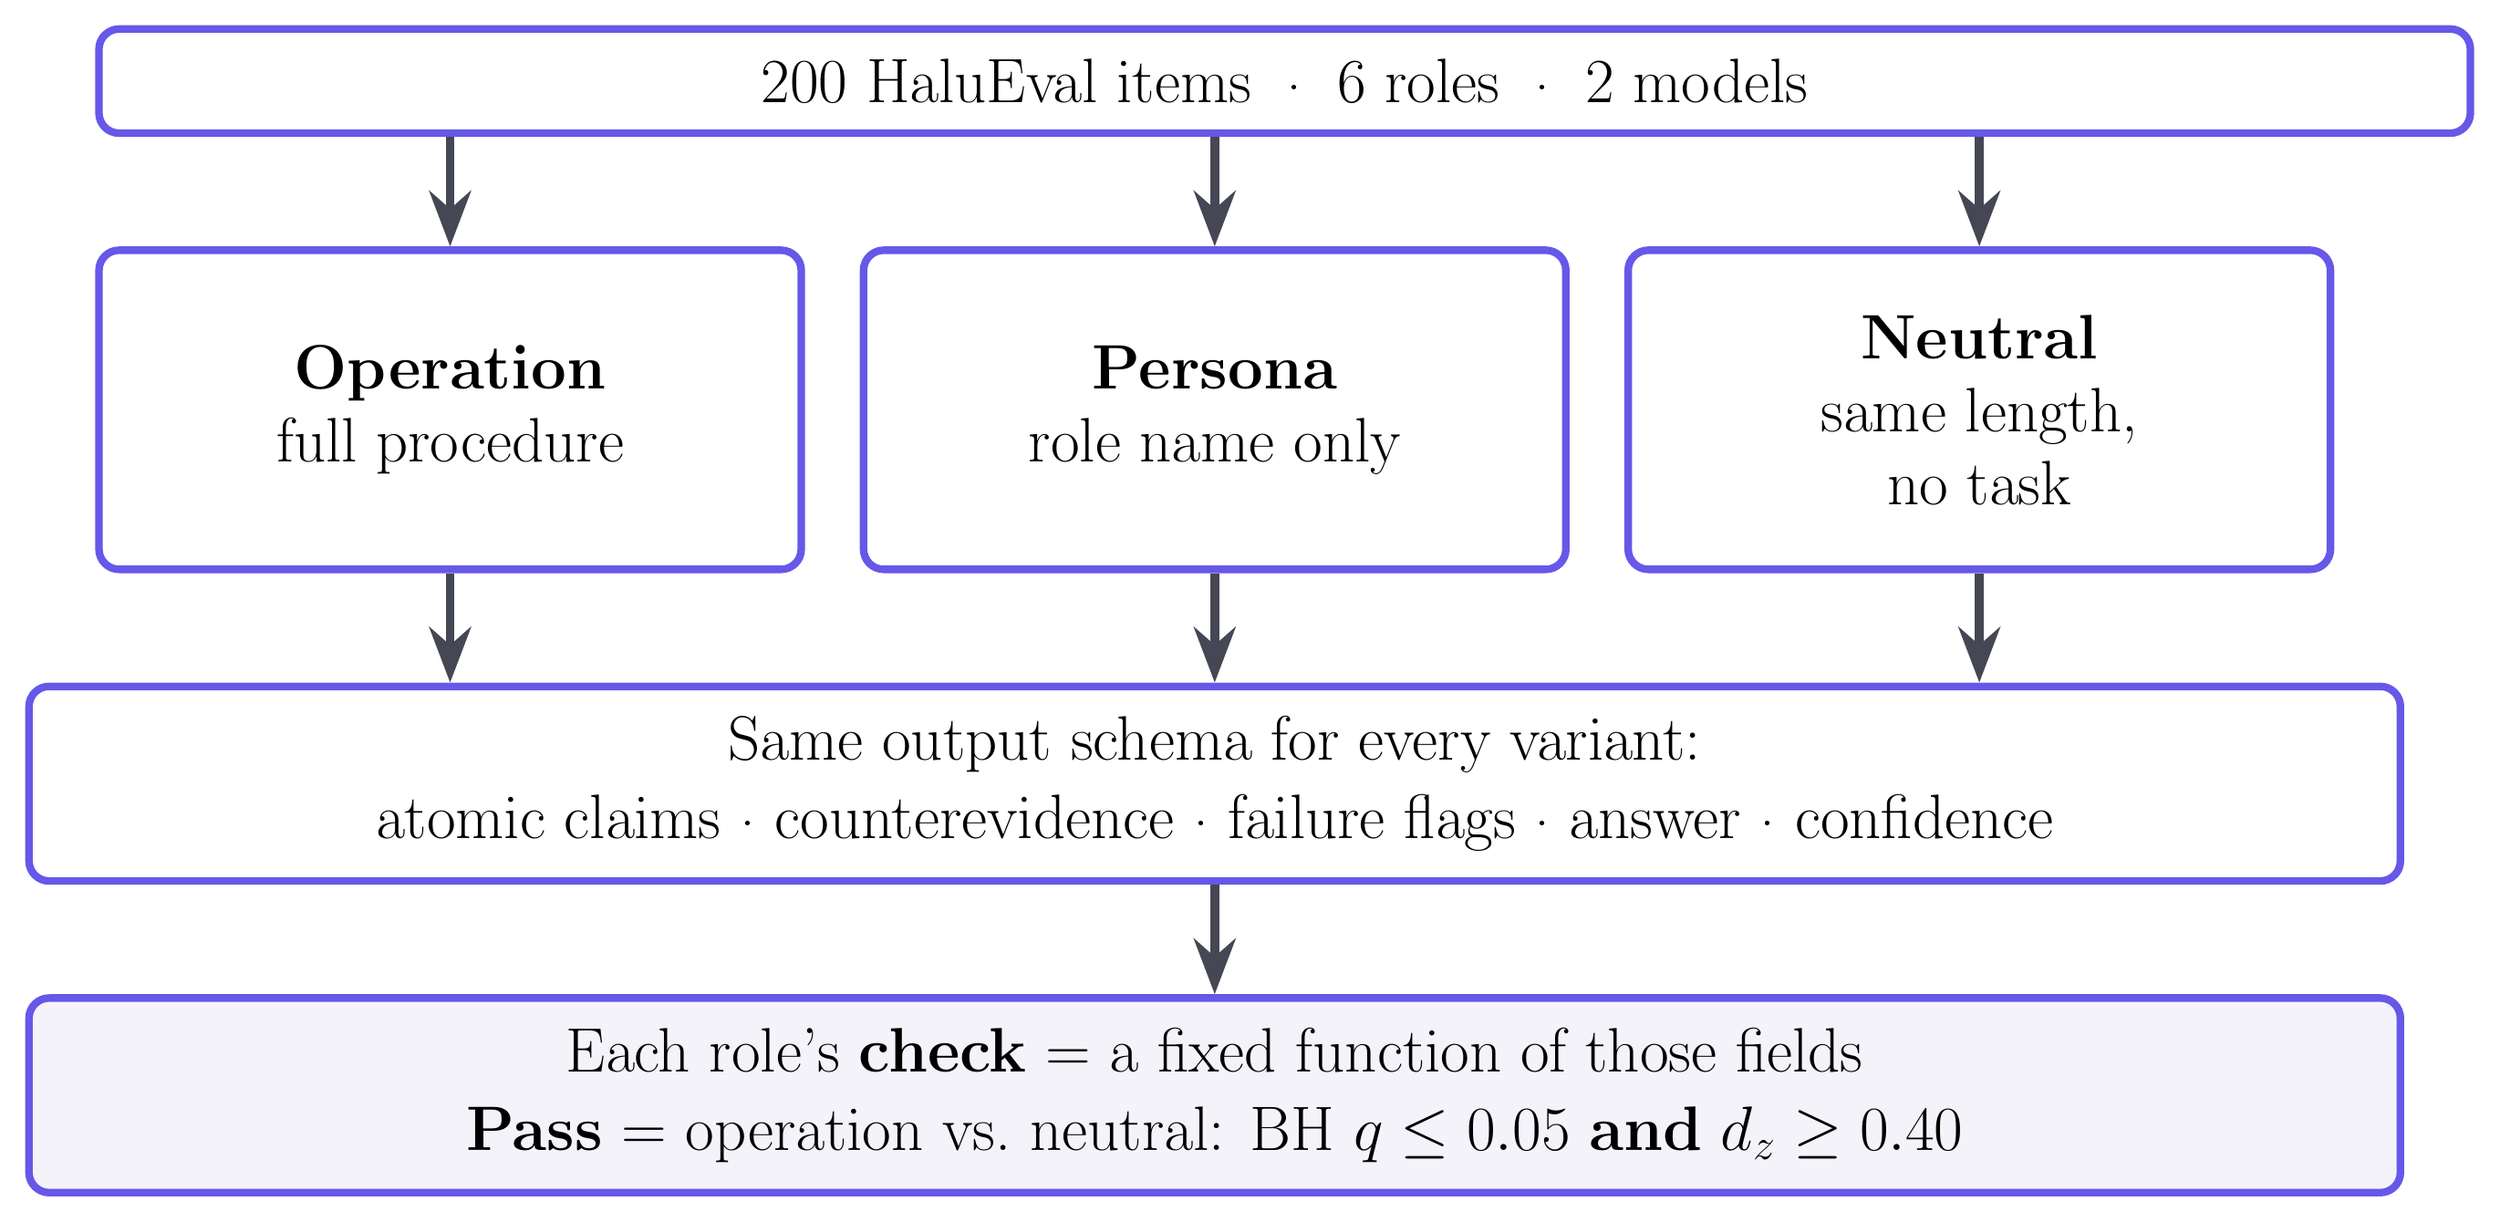
\begin{tikzpicture}[font=\fontsize{25}{31}\selectfont, node distance=0.55in,
  box/.style={draw=accent, line width=3pt, rounded corners=8pt, fill=white,
    align=center, inner sep=12pt},
  var/.style={box, minimum width=3.85in, minimum height=1.75in},
  arr/.style={-{Stealth[length=22pt]}, line width=3.5pt, color=secondary}]
  \node[box, minimum width=13in] (item) {200 HaluEval items \;·\; 6 roles \;·\; 2 models};
  \node[var, below=0.6in of item.south west, anchor=north west] (op)
    {\textbf{Operation}\\[-2pt]full procedure};
  \node[var, right=0.3in of op] (pe) {\textbf{Persona}\\[-2pt]role name only};
  \node[var, right=0.3in of pe] (ne) {\textbf{Neutral}\\[-2pt]same length,\\[-2pt]no task};
  \foreach \n in {op,pe,ne} \draw[arr] (item.south -| \n.north) -- (\n.north);
  \node[box, below=0.6in of pe, minimum width=13in] (schema)
    {Same output schema for every variant:\\ atomic claims · counterevidence · failure flags · answer · confidence};
  \foreach \n in {op,pe,ne} \draw[arr] (\n.south) -- (\n.south |- schema.north);
  \node[box, below=0.6in of schema, minimum width=13in, fill=tint] (chk)
    {Each role's \textbf{check} = a fixed function of those fields\\
     \textbf{Pass} = operation vs.\ neutral: BH $q \le 0.05$ \textbf{and} $d_z \ge 0.40$};
  \draw[arr] (schema) -- (chk);
\end{tikzpicture}
\end{center}
\vspace{-0.2em}
{\smalltext
\begin{itemize}
\item \textbf{Task:} HaluEval QA. Given a knowledge passage, does a candidate answer contain hallucinated content? (yes/no)
\item \textbf{Models:} \texttt{gpt-5.6-terra} (primary), \texttt{grok-4.3} (replication). Temperature 0, seed 1337, one sample per item.
\item \textbf{Scale:} 3,600 calls per model, 0 refusals, 0 exclusions.
\item \textbf{Statistics:} $d_z$ = mean paired difference / SD of differences; 2,000-resample paired bootstrap; BH across the six roles. Rule fixed before data.
\end{itemize}}

\vspace{0.5em}
\sect{3}{The six checks, and what their guards did}
{\fontsize{25.5}{34}\selectfont
\renewcommand{\arraystretch}{1.3}
\begin{tabularx}{\linewidth}{@{}>{\bfseries}p{2.9in}X@{}}
\toprule
Role & What the check computes $\;\rightarrow\;$ what happened to its guard \\
\midrule
Counter-\newline evidence & \# counterclaims + \# claims marked unsupported or contradicted.
  \newline\textcolor{secondary}{No guard: any counterclaim counts, whatever its quality.} \\
Consistency & Rate of contradiction or calculation-error flags $-$ abstention rate.
  \newline\textcolor{secondary}{Defeatable: flag everything and still answer to score 1.0.} \\
Local-claim & \# claims $\times$ (1 + share with a source).
  \newline\textcolor{secondary}{Models self-report a source on 99\% of claims, so the factor is 2 on 1,191 of 1,200 records: the check is 2 $\times$ claim count.} \\
Explore-then-\newline prune & \# distinct claims $\times$ (1 $-$ share marked uncertain).
  \newline\textcolor{secondary}{Only 0.5--1.7\% of claims are uncertain, so the factor is $\approx$1.} \\
Rare-\newline hypothesis & \# supported claims with a source $-$ \# without.
  \newline\textcolor{secondary}{Penalty almost never fires (1 of 7,638 claims on terra).} \\
Confidence\newline calibration & $-$ECE over stated confidences (10 equal-mass bins).
  \newline\textcolor{secondary}{Defeatable on terra: lowering every confidence by 0.05 cuts ECE from 0.144 to 0.112 (no shift helps on grok).} \\
\bottomrule
\end{tabularx}}
\end{minipage}%
\hspace{0.7in}%
% ---------------------------------------------------------------- column 2
\begin{minipage}[t]{18.4in}
\sect{4}{Verdicts: one role passes on terra, two on grok}
\begin{minipage}[t]{11.4in}\vspace{0pt}
\includegraphics[width=\linewidth]{figures/fig_verdicts.pdf}
\end{minipage}\hfill
\begin{minipage}[t]{6.6in}\vspace{0.3in}
\begin{callout}
{\color{terra}\textbf{terra:}} only counter-evidence passes ($d_z = +1.03$; counterclaims
plus flags rise from 0.61 to 1.285 per answer).

\vspace{0.3em}
{\color{grok}\textbf{grok:}} counter-evidence ($+0.52$) and local-claim ($+0.69$).

\vspace{0.3em}
\textbf{Bare role names} barely move their own checks: $|d_z| \le 0.30$ on both models.

\vspace{0.3em}
\textbf{Explore-then-prune} goes \emph{down}: $-0.95$ and $-1.66$.
\end{callout}
\end{minipage}

\vspace{0.4em}
\sect{5}{Auditing the instrument}
\textbf{Three checks are claim counters.} Local-claim is exactly
2 $\times$ claim count on this data. Explore-then-prune and rare-hypothesis follow
claim count closely. That redundancy comes from how the checks are defined, not
from what the prompts do.
\par\vspace{0.1em}
\includegraphics[width=\linewidth]{figures/fig_claimcount.pdf}

\vspace{0.2em}
\textbf{Do prompts move only their own check?} Each row is a prompt; each column
is a check ($d_z$ vs.\ neutral; diagonal outlined). A role is
\emph{specific} if its own effect beats every other by $\ge$ 0.20, a criterion
fixed before we computed the matrix. \textbf{This holds in 1 of 12 cells.}
\par\vspace{0.1em}
\includegraphics[width=\linewidth]{figures/fig_matrix.pdf}
\end{minipage}%
\hspace{0.7in}%
% ---------------------------------------------------------------- column 3
\begin{minipage}[t]{12.6in}
\sect{6}{What the audit means}
\begin{callout}
\textbf{The explore-then-prune reversal is an artifact.} The prompt says:
\par\vspace{0.2em}
{\itshape\color{secondary}``Record the \textbf{surviving} hypotheses as atomic claims.''}
\par\vspace{0.2em}
The check counts recorded claims as first-pass breadth, so fewer claims is what
the prompt asks for, not evidence of less exploration.
\end{callout}
\vspace{0.2em}
\begin{callout}
\textbf{Three guards were never tested, not proven broken.} The behaviour they
guard against (unsourced, uncertain, or fabricated claims) barely occurred. But
``sourced'' is the model's own report, so these guards check self-reports.
\end{callout}
\vspace{0.2em}
\begin{callout}
\textbf{Direction matters.} Counting only effects in the \emph{same} direction (an
opposite effect may be a trade-off), counter-evidence clears the margin on both
models ($+0.77$, $+0.52$); nothing else does. \emph{Sensitivity analysis added after review.}
\end{callout}

\vspace{0.4em}
{\fontsize{30}{38}\selectfont\bfseries Councils do not beat a single call\par}
\vspace{0.1em}
{\smalltext 1,000 HaluEval items, \texttt{gpt-5.6-terra}, majority vote. Accuracy
0.846 / 0.846 / 0.839 vs.\ 0.861. Gains above 0.6 points are ruled out under
both tie rules.\par}
\includegraphics[width=\linewidth]{figures/fig_council.pdf}

\vspace{0.3em}
\begin{keybox}
{\fontsize{33}{42}\selectfont\bfseries No role has a validated pass.\par}
\vspace{0.3em}
The only terra pass is an unguarded raw count; the grok local-claim pass is a
claim counter. A benchmark delta does not show a role did its job, and
\textbf{neither does a manipulation check until the check itself is tested.}
\end{keybox}

\vspace{0.4em}
{\fontsize{30}{38}\selectfont\bfseries Next\par}
{\smalltext
\begin{itemize}
\item \textbf{Sensitivity:} preregistered positive (worked example) and negative (``avoid it'') controls for every check.
\item \textbf{Convergent validity:} judge or human ratings of whether counterclaims are substantive.
\item \textbf{Better checks:} normalize by claim count; record first-pass hypotheses.
\item \textbf{Scope:} reworded prompts and a third, open-weight model. Today: six roles, one council design, one benchmark, two models.
\end{itemize}}

\vspace{0.5em}
{\tinytext\color{secondary}\textbf{References.}
Hauser, Ellsworth \& Gonzalez (2018), \emph{Are manipulation checks necessary?} Front.\ Psychol.\ \textbullet\
Ejel\"ov \& Luke (2020), \emph{``Rarely safe to assume''}, J.\ Exp.\ Soc.\ Psychol.\ \textbullet\
Cemri et al.\ (2025), \emph{Why do multi-agent LLM systems fail?} NeurIPS \textbullet\
Zheng et al.\ (2024), \emph{When ``A Helpful Assistant'' is not really helpful}, Findings of EMNLP \textbullet\
Dietrich (2026), \emph{When roles fail}, arXiv:2604.27228 \textbullet\
Li et al.\ (2023), \emph{HaluEval}, EMNLP.\par}
\end{minipage}

\vfill
{\tinytext\color{secondary}
\textbf{Contact:} zhouk.2009@gmail.com, sparshr@mit.edu, maximkud21+research@gmail.com \quad·\quad Code, records and this poster: \textbf{github.com/kevzho/role-prompted-systems}
\quad·\quad Exploratory analyses (Sections 5--6) were computed on already-observed records.
\quad·\quad Model inference funded by Microsoft for Startups Azure credits.\par}
\end{document}
